\documentclass[tikz,border=2pt]{standalone}
\usepackage{newpxtext,newpxmath}
\definecolor{curve}{HTML}{1f6fb2}
\definecolor{accent}{HTML}{c0392b}
\definecolor{polygon}{HTML}{555555}
\definecolor{muted}{HTML}{dfe6ee}
\begin{document}
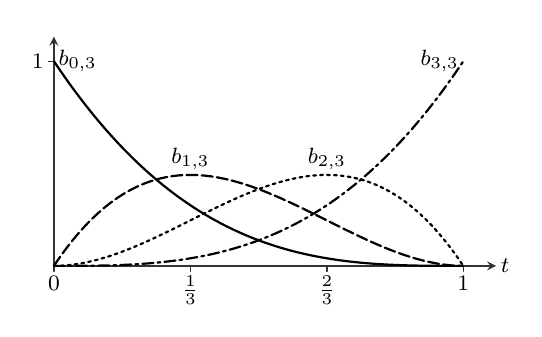
\begin{tikzpicture}[
  x=5.2cm, y=2.6cm,
  line cap=round, line join=round,
  every node/.style={font=\footnotesize, inner sep=1.5pt},
  curve/.style={draw=curve, line width=1.1pt},
  second/.style={draw=accent, line width=1.1pt},
  polygon/.style={line width=0.5pt, dash pattern=on 2.5pt off 2pt},
  construction/.style={draw=accent, line width=0.5pt},
  axis/.style={line width=0.45pt, draw=black!80, >=stealth},
  ctrl/.style={circle, fill=white, line width=0.6pt, minimum size=4pt, inner sep=0pt},
]
\draw[axis, ->] (0,0) -- (1.08,0) node[right] {$t$};
\draw[axis, ->] (0,0) -- (0,1.12) node[above] {};
\draw[axis] (0,0) -- ++(0,-2pt) node[below] {$0$};
\draw[axis] (0.3333,0) -- ++(0,-2pt) node[below] {$\frac13$};
\draw[axis] (0.6667,0) -- ++(0,-2pt) node[below] {$\frac23$};
\draw[axis] (1,0) -- ++(0,-2pt) node[below] {$1$};
\draw[axis] (0,1) -- ++(-2pt,0) node[left] {$1$};
\draw[draw=black, line width=0.8pt, ] (0.0000,1.0000) .. controls (0.3333,0.0000) and (0.6667,0.0000) .. (1.0000,0.0000);
\node[right] at (0,1) {$b_{0,3}$};
\draw[draw=black, line width=0.8pt, dash pattern=on 4pt off 1.5pt] (0.0000,0.0000) .. controls (0.3333,1.0000) and (0.6667,0.0000) .. (1.0000,0.0000);
\node[above] at (0.3333,0.4444) {$b_{1,3}$};
\draw[draw=black, line width=0.8pt, dash pattern=on 1pt off 1.5pt] (0.0000,0.0000) .. controls (0.3333,0.0000) and (0.6667,1.0000) .. (1.0000,0.0000);
\node[above] at (0.6667,0.4444) {$b_{2,3}$};
\draw[draw=black, line width=0.8pt, dash pattern=on 4pt off 1.5pt on 1pt off 1.5pt] (0.0000,0.0000) .. controls (0.3333,0.0000) and (0.6667,0.0000) .. (1.0000,1.0000);
\node[left] at (1,1) {$b_{3,3}$};
\end{tikzpicture}
\end{document}
